\chapter{A Graph Theoretic Approach to Constructing Room Squares}

\section{Graph factorisations}

A graph $G(V,E)$ consists of two sets. The first $V$,
is called the vertex-set, while the other $E$ consists
of unordered pairs of $V$ and is called the edge set.
Usually graphs are represented with diagrams where the
members of $V$ are drawn as points and the members of
$E$ as lines connecting points. Adjacency for two vertices
means being connected by an edge. The
\emph{complete graph}
$K_n$ is the graph on $n$ vertices in which all distinct
vertices are adjacent.

\begin{figure}
  \begin{centering}
    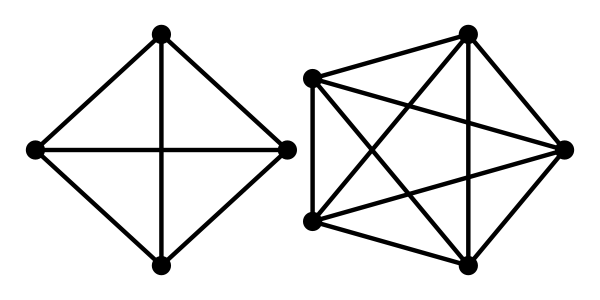
\includegraphics[width=0.8\textwidth, center]{figure/complete_graph.png}
  \end{centering}
\end{figure}

A
\emph{one-factor}
$f_i$ is a set of edges in which each vertex
appears exactly once.

\begin{example}
Two possible one-factors of $K_4$ are:
$$f_1 = \{12,34\},\, f_2 = \{13,24\}$$
\end{example}

\begin{figure}
  \begin{centering}
    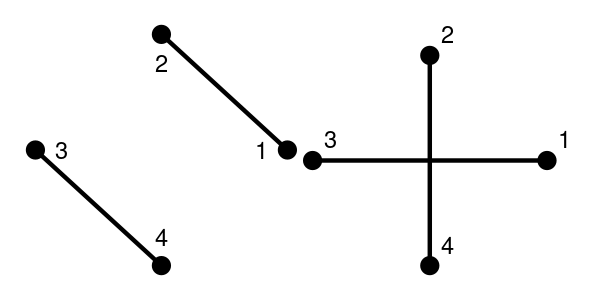
\includegraphics[width=0.8\textwidth, center]{figure/two_one_factors.png}
  \end{centering}
\end{figure}

A
\emph{one-factorisation}
of the complete graph is a set of
one-factors in which all possible edges (i.e. all unordered
pairs from the edge-set) appear exactly once.

\begin{figure}
  \begin{centering}
    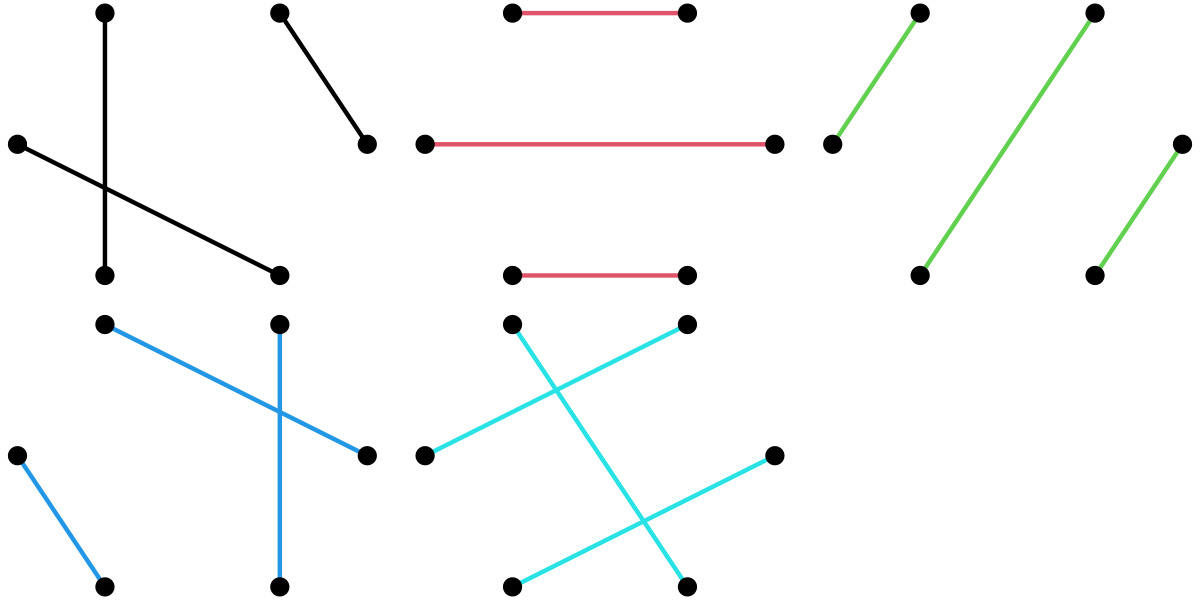
\includegraphics[width=0.8\textwidth, center]{figure/one_factorisation.png}
  \end{centering}
\end{figure}

\begin{example}
Here
$G = K_6$
the complete graph on six vertices with
$$V = \{1, 2, 3, 4, 5, 6\}$$
$$E = \{12, 13, 14, 15, 16, 23, 24, 25, 26, 34, 35, 36, 45, 46, 56\}$$
The one-factors are

$$
f_1 = \{12, 35, 46\} \hspace{0.5cm}
f_2 = \{14, 23, 56\} \hspace{0.5cm}
f_3 = \{16, 25, 34\} \hspace{0.5cm}
f_4 = \{13, 26, 45\} \hspace{0.5cm} 
f_5 = \{15, 24, 36\}
$$
because
$f_1 \cup f_2 \cup f_3 \cup f_4 \cup f_5 = E$,
$F = \{f_1, f_2, f_3, f_4, f_5\}$
is a one-factorisation of
$G$,
shown in Figure~\ref{fig:one-factorisation}.
\end{example}

Two one factors $f$ and $l$ are said to be
\emph{orthogonal}
if $f \cap l$ contains at most one edge. Two one-factorisations
$F$ and $L$ are orthogonal if every one-factor in $F$ is
orthogonal to every one-factor in $L$.

Once again consider the square array in
\eqref{eq:roomsquare}.
If the individual elements within the array constituted the
vertex set of a graph (call it $R$) and the pairs within
each box of the array were edges, we know that each row is a
one-factor and each column is a one-factor (because each
member of $R$ occurs precisely once in each row and once in
each column).

Furthermore, because all edges from the
edge-set of the complete graph (i.e. all unordered pairs
from $R$) appear once within the array, we know that the
rows together form a one-factorisation and the columns form
another, different, one-factorisation of $K_8$. Also,
because any row factor intersects any column factor in only
one pair (edge), all the row factors are orthogonal to all
the column factors and hence the two one-factorisations are
orthogonal. We have demonstrated the following theorem,
given in
\cite{dinitzContemporaryDesignTheory1992}
and proven in
\cite{nemethStudyRoomSquares1969}.

\begin{theorem}
The existence of a Room square of side $n$
is equivalent to the existence of two orthogonal
one-factorisations of the complete graph $K_{n+1}$.
\end{theorem}

An example is given in Figure
\ref{fig:orthogonal}
based on the Room square
in 
\eqref{eq:roomsquare}

\begin{figure}
  \begin{centering}
    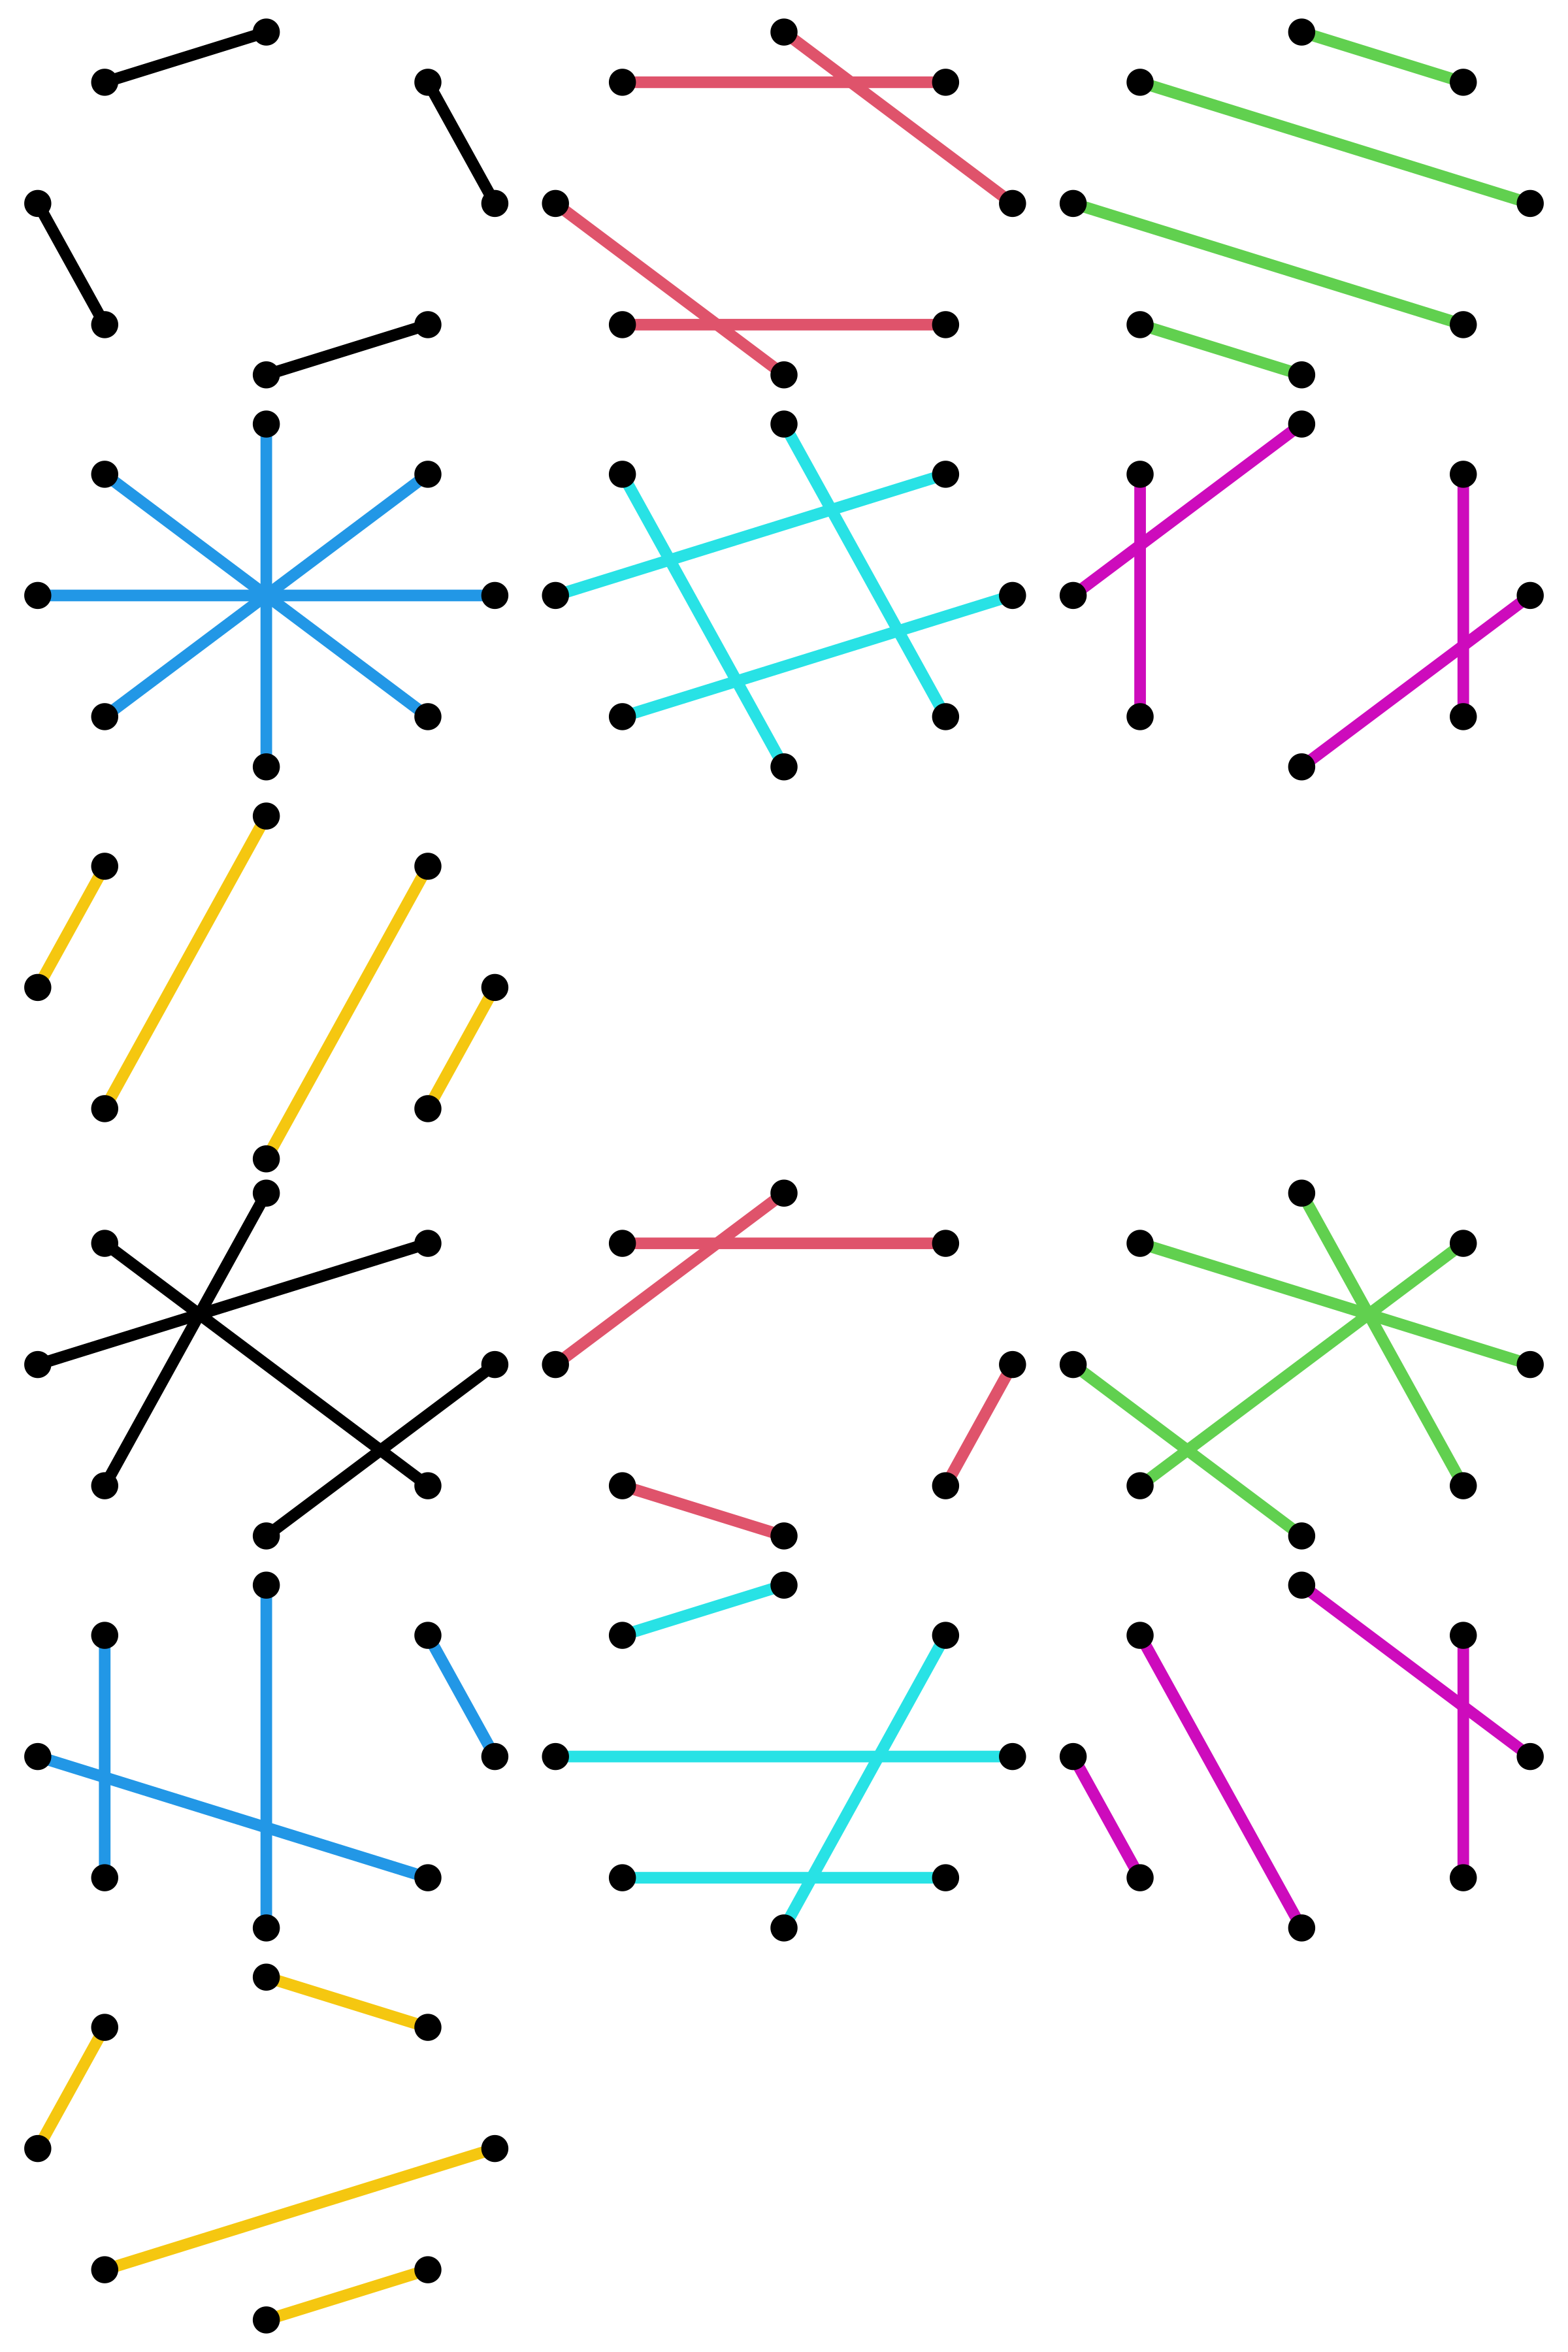
\includegraphics[width=0.8\textwidth, center]{figure/orthogonal_one_factorisation.png}
  \end{centering}
\end{figure}

\section{Hill-Climbing Algorithm for Room Squares}

The idea behind hill-climbing algorithms is to suppose
there exists a
\emph{neighbourhood}
of feasible solutions to
some problem
\emph{instance}.
With each
\emph{feasible}
solution
there is an associated
\emph{cost}
(or profit) and finding
an optimal solution becomes a matter of finding the solution
with minimum cost (or maximum profit).

A hill-climbing algorithm non-deterministically selects a
solution from the neighbourhood system such that the cost
is less than that of some initial solution until its
procedure fails, hence finding the locally optimal solution.

\subsection{An algorithm for one-factorisations}

Consider how to find a one-factorisation of the complete
graph. Here the problem instance is simply the even integer
$n$ and vertex set $V$.

Recall:
\begin{itemize}
  \item{A one-factor of $K_n$ is a set of $n/2$ edges (hence $n$ is even) which partition $V$.}
  \item{A one-factorisation of $K_n$ is a set of $n - 1$ one-factors which partitions the edge set of $K_n$.}
\end{itemize}

Suppose we choose to represent a one-factorisation by a set
of $\frac{n}{2}(n - 1) = (n^2 - n)/2$ pairs each of the form
$(f_i, \{x, y\})$, where $x \neq y, i = 1 \ldots n - 1$,
and the following two conditions hold:
\begin{enumerate}
  \item{Every $\{x, y\}$ occurs in a unique pair $(f_i, \{x, y\})$.}
  \item{For every one-factor $f_i$ and every vertex $x$, there is a unique pair of the form $(f_i, \{x, y\})$.}
\end{enumerate}
where $f_i$s are one-factors.

Then we consider a feasible solution to be a partial
one-factorisation, again represented by pairs having the
same form but this time,

\begin{enumerate}
  \item{Every $\{x, y\}$ occurs in at most one pair $f_i, \{x, y\})$.}
  \item{For every one-factor $f_i$ and every vertex $x$ there is at most one pair of the form $(f_i, \{x, y\})$.}
\end{enumerate}

Where the $f_i$s are
\emph{partial one-factors}.

Which enables a definition for the cost of a feasible solution $F$ to be given by:

$$c(F) = (n^2 - n)/2 - |F|$$

So that $F$ is a one-factorisation if and only if $c(F) = 0$, i.e. $|F| = (n^2 - n)/2$

Now suppose that we can implement some procedure $X$, say,
which either reduces the cost or leaves it unaffected
(i.e. it never increases the cost) then the following
``hill-climbing'' algorithm, provided it terminates,
will find a one-factorisation.

\begin{algorithm}[H]
  \While{$c(F) \neq 0$}{$X$}
\end{algorithm}

A procedure such as $X$ is called a heuristic.
The following two heuristics from
\cite{dinitzHillClimbingAlgorithmConstruction1987}
when used together are suitable for finding a
one-factorisation.

Let $F$ be a partial one-factorisation of $K_n$:

\begin{algorithm}[H]
\KwIn{any vertex $x$ such that $x$ does not occur in 
     every partial one-factor of $F$ (such a vertex is said
     to be a live point)}
\KwIn{any partial one-factor $f_i$ such that $x$ does
     not occur in $f_i$}
\KwIn{any $y \neq x$ such that there is no partial
     one-factor $f_j$ for which $(f_j,\{x,y\}) \in F$
     (we say that $x$ and $y$ do not occur together).}
\eIf{$y$ does not occur in $f_i$}{
  replace $F$ with $F \cup \{(f_i,\{x,y\})\}$
}{
  there is a pair in $F$ of the form $(f_i,\{z,y\}) (z \neq x)$.
  Replace $F$ with
    $F \cup \{(f_i,\{x,y\})\} \backslash \{(f_i,\{z,y\})\}$
}
\caption{$H_1$}
\end{algorithm}

\begin{algorithm}[H]
\KwIn{any partial one-factor $f_i$ which does not
     occur in exactly $n/2$ pairs in $F$ (such a partial
     one-factor is said to be live)}
\KwIn{any $x$ and $y$ such that $x$ and $y$ do not 
     occur together in $f_i$}
\eIf{$x$ and $y$ do not occur together}{
 Replace $F$ with $F \cup \{(f_i, \{x, y\})\}$
}{there is a pair in $F$ of the form $(f_j,\{x, y\}) (j \neq i)$.
  Replace $F$ with
    $F \cup \{(f_i,\{x,y\})\} \backslash \{(f_j,\{x,y\})\}$ }
\caption{$H_2$}
\end{algorithm}

\begin{example}
Suppose we are in the process of trying to find a
one-factorisation for $K_6$, and have generated a partial
one-factorisation represented by the set $F$.

\begin{equation*}
F = \{(f_1,\{4,6\}),(f_1,\{3,5\}),(f_2,\{5,6\}),(f_3\{1,6\}), (f_3\{3,4\}),(f_4,\{2,3\}),(f_4,\{4,5\})\}
\end{equation*}

Now apply $H_1$.

\begin{enumerate}
  \item{Choose $x = 2$. Live, because it doesn’t appear in $f_1, f_2, f_3$ or $f_5$.}
  \item{Of these four partial one factors, choose $f_1$.}
  \item{2 only occurs together with 3 (in $f_4$), so pick $y = 5$.}
  \item{5 already appears in $f_1$ so $\{z, y\} = \{3, 5\}$.
     So replace $F$ by
     $F \cup \{(f_1, \{2, 5\}) \backslash (f_1, \{3, 5\})\}$}
\end{enumerate}

So we have extracted one edge from the one-factorisation and
replaced it with another edge, leaving the cost unchanged.

If in 3. we had picked 1 then according to the heuristic we
should replace $F$ with $F \cup (f_1, \{2, 1\})$, increasing
$|F|$ by one, and so decreasing the cost by the same. Because
the cost cannot increase $H_1$ is a suitable heuristic for use
in a hill-climbing algorithm.

Now apply $H_2$ to the new one-factorisation
$F_1 = F \cup (f_1, \{2, 1\})$.

\begin{enumerate}
  \item{We can pick any of $f_2, f_3, f_4, f_5$, because all are live. Choose $f_2$.}
  \item{Choose $x = 2, y = 3$, because neither appear in $f_2$.}
  \item{2 and 3 occur together in $f_4$. So replace $F_1$
     with
     $F_1 \cup \{(f_2, \{2, 3\}) \backslash (f_4, \{2, 3\})\}$}
\end{enumerate}

Again the cost remains unchanged by this procedure,
and if in 2, we had chosen $x = 1, y = 4$ instead then
we would have replaced $F_1$ with
$F_1 \cup \{(f_2, \{1, 4\})\}$
decreasing the cost by one. As with $H_1$,
the cost cannot increase, which makes $H_2$ a suitable
heuristic.
\end{example}

The hill-climbing algorithm for constructing one-factorisations
which was first given in
\cite{dinitzHillClimbingAlgorithmConstruction1987}
has a very simple form.

\begin{algorithm}[H]
\While{$c(F) \neq 0$}{
  choose $r = 1$ or $r = 2$ with equal probability
  perform $H_r$}
\end{algorithm}

\subsection{An algorithm for Room squares}

To generate a Room square all that remains is to produce
another one-factorisation $G$, say, which is orthogonal to
$F$. This will inevitably require slight modifications to
be made to $H_1$ and $H_2$.

Now if an array $R$ is constructed in which the rows are
labelled with the one-factors of $F(f_1,f_2,...,f_{n-1})$,
and the columns are labelled with the partial one-factors
of $G(g_1,g_2,...,g_{n-1})$. Then $R$ will be a Room square
if the $(f_i,g_j)$ cell contains $\{x,y\}$, if and only if
$(f_i,\{x,y\}) \in F$ and $(g_j,\{x,y\}) \in G$ and is empty
otherwise.

Again these two heuristics are due to Dinitz and Stinson and
originally presented in
\cite{dinitzHillClimbingAlgorithmConstruction1987}.
Although a necessary correction has been made as will
become apparent.

\begin{algorithm}[H]
  1. Choose any live point $x$.

  2. Choose any partial one-factor $g_i$ such that $x$ does
     not occur in $g_i$.

  3. Choose any $y \neq x$ such that $x$ and $y$ do not occur
     together in $G$.

  4. Let $f_j$ be the one-factor of $F$ which contains the 
     edge $\{x, y\}$.
     
  \uIf{$R(f_j, g_i)$ is not empty}{
    $OH_1$ fails \;
  }
  \uElseIf{$y$ does not occur in $g_i$}{
    Replace $G$ by $G \cup (g_i, \{x, y\})$.

    Define $R(f_j, g_i)=\{x, y\}$.
  }
  \Else{
    there is a pair in $G$ of the form
     $(g_i, \{z, y\}) \hspace{0.5cm} z \neq x$.

    Replace $G$ by
    $G \cup (g_i, \{x, y\}) \backslash (g_i, \{z, y\})$.

    Define $R(f_k, g_i)$, to be empty$^i$,
    where $(f_k, \{z, y\}) \in F$.
  }
\caption{$OH_1$}
\end{algorithm}

\begin{algorithm}[H]
  1. Choose any live partial one-factor $g_i$.

  2. Choose any $x$ and $y \neq x$ such that $x$ and $y$
     do not occur together in $g_i$.

  3. Let $f_j$ be the one-factor of $F$ which contains
     the edge $\{x, y\}$.
  
  \uIf{$R(f_j, g_i)$ is not empty}{
    $OH_2$ fails
  }
  \uElseIf{$x$ and $y$ do not occur together}{
   Replace $G$ by $G \cup (g_i, \{x, y\})$.

   Define $R(f_j, g_i) = \{x, y\}$.
  }
  \Else{
    there is a pair in $G$ of the form
    $(g_k, \{x, y\}) \hspace{0.5cm} (k \neq i$)

       Replace $G$ by
       $G \cup (g_i, \{x, y\}) \backslash (g_k, \{x, y\})$

       Define $R(f_j, g_i) = \{x, y\}$.

       Define $R(f_j, g_k)$ to be empty.
  }
\caption{$OH_2$}
\end{algorithm}

\begin{example}
Suppose the factorisation $F$ from the earlier example has
been completed and is represented by the set:

\begin{equation}
  \begin{split}
    F = \{(f_1\{1,2\}),(f_1\{3,5\}),(f_1\{4,6\}),(f_2\{1,4\}),(f_2\{2,3\}),(f_2\{5,6\}), \\
    (f_3\{1,6\}),(f_3\{2,5\}),(f_3\{3,4\}),(f_4\{1,3\}),(f_4\{2,6\}),(f_4\{4,5\}),(f_5\{1,5\}),(f_5\{3,6\})\}
  \end{split}
\end{equation}

Notice that this is precisely the one-factorisation of $K_6$
given on page XXX.

Now suppose we have established the following one-factors in
$G$:

\begin{equation}
  G = \{(g_1, \{1, 4\}), (g_2, \{1, 6\}), (g_3, \{3, 6\}), (g_5\{5, 6\}), (g_5\{1, 2\})\}
\end{equation}

At this state $R$ looks like 

\begin{equation}
  \begin{bmatrix}
     -  &   g_1    &    g_2    &    g_3   & g_4 &    g_5    \\
    f_1 &     -    &     -     &    -     &  -  & \{1, 2\}  \\
    f_2 & \{1, 4\} &     -     &    -     &  -  & \{5, 6\}  \\
    f_3 &     -    &  \{1, 6\} &    -     &  -  &     -     \\
    f_4 &     -    &     -     &    -     &  -  &     -     \\
    f_5 &     -    &     -     & \{3, 6\} &  -  &     -     \\
  \end{bmatrix}
\end{equation}

Now apply $OH_1$:

\begin{enumerate}
  \item{Choose $x = 5$, suitably live.}
  \item{Choose $g_3$, in which $5$ does not occur.}
  \item{$5$ does not occur together with $2$ in $G$, so we are
     free to choose $y = 2$.}
  \item{In $F$, $\{2, 5\} \in f_3$.}
  \item{
    $f_3, g_3$ is empty in $R$, also $y = 2 \notin g_3$.
    \begin{itemize}
       \item{Replace $G$ with $G \cup (g_3, \{5, 2\})$.}
       \item{Define $R(f_3, g_3) = \{5, 2\}$.}
    \end{itemize}
  }
\end{enumerate}

This decreases the cost by one, alternatively we might have
chosen, at stage 3. $y = 3$, in that case.

\begin{enumerate}
  \setcounter{enumi}{4}
  \item{$\{3, 5\} \in f_1$.}
  \item{
    $f_1, g_3$ is empty in $R$, also $y \in g_3$, occurring
      in the pair $(g_3, \{3, 6\}), z = 6$.
    \begin{itemize}
      \item{Replace $G$ with
        $G \cup (g_3, \{3, 5\}) \backslash (g_3, \{3,
        6\})$.}
      \item{Define $R(f_1, g_3) = \{3, 5\}$.}
      \item{Define $R(f_5, g_3)$ to be empty.}
    \end{itemize}
  }
\end{enumerate}

Which leaves the cost unaffected. Suppose now that $R$ is the
array after this second version of the application of $OH_1$:

\begin{equation}
  \begin{bmatrix}
     -  &   g_1    &    g_2    &    g_3   & g_4 &    g_5    \\
    f_1 &     -    &     -     & \{3, 5\} &  -  & \{1, 2\}  \\
    f_2 & \{1, 4\} &     -     &    -     &  -  & \{5, 6\}  \\
    f_3 &     -    &  \{1, 6\} &    -     &  -  &     -     \\
    f_4 &     -    &     -     &    -     &  -  &     -     \\
    f_5 &     -    &     -     &    -     &  -  &     -     \\
  \end{bmatrix}
\end{equation}

Now if we apply $OH_2$:

\begin{enumerate}
  \item{Choose $g_4$, a live partial one-factor.}
  \item{Choose $x = 1, y = 2$, neither of which occur in $g_4$.}
  \item{$(f_1, \{1, 2\}) \in F$.}
  \item{
    $f_1, g_4$ is empty in $R$, also $x$ and $y$ do occur
    together, $(g_5, \{1, 2\}) \in G$.
    \begin{itemize}
      \item{Replace $G$ with
       $G \cup (g_4, \{1, 2\}) \backslash (g_5, \{1, 2\})$}
      \item{Define $R(f_1, g_4) = \{1, 2\}$.}
      \item{Define $R(f_1, g_5)$ to be empty.}
    \end{itemize}
  }
\end{enumerate}

This procedure leaves the cost unaffected and if instead we had
chosen at $2$. $x = 3, y = 4$, then would have been required to
replace $G$ with $G \cup (g_4,\{3,4\})$, and put $\{3, 4\}$ in
cell $(f_3, g_4)$ of $R$, an action which reduces the cost by one.
However, we know that two orthogonal one-factorisations of $K_6$
are equivalent to a Room square of side 5, which has been shown
not to exist. Hence it would be futile to continue with this
method in this particular case. Nevertheless the example shows
how the heuristics work.
\end{example}

There is no guarantee of success with repeated use of these
heuristics, although Dinitz and Stinson are quick to point out that
the algorithm involving $H_1$ and $H_2$ has never
\footnote{In over ten-million attempts, they claim.}
failed to
produce the desired one-factorisation. If we hope to use the
$OH_1$ and $OH_2$ in a similar algorithm then the possibility of
failure becomes a real possibility.

Two possibilities exist, either both heuristics fail or
successive use of them leads to an infinite loop. In order to
avoid both we introduce a
\emph{threshold}
function which simply
arrests the progress of the algorithm after a certain number of
iterations of the heuristics. Dinitz and Stinson found after
experimentation that the following function is suitable.

\begin{equation}
T(n) = 100n
\end{equation}

Then the hill-climbing algorithm for finding a Room square is as
follows:

\begin{algorithm}[H]
\KwIn{Use the previous hill climbing algorithm to construct $F$,
     a one-factorisation of $K_n$.}
\KwIn{Number of iterations initialised to be $0$}
\While{(number of iterations $<T(n)$) and $c(G) \neq 0$}{
   Choose $r = 1$ or $r = 2$ at random with equal probability.
   Perform $OH_r$.
   Increment number of iterations.}
\end{algorithm}

\subsection{The Room Square Generator}

Dinitz and Stinson choose to implement the above algorithm in
Pascal, and ran in on an Amdahl 5850 workstation. It was very
successful, finding many Room squares with sides ranging from 11
to 101. For each successful trial they had 9 or 10 failures (the
program being stopped by the threshold function) and timings
ranged from 0.09 seconds for an
$11 \times 11$
Room square, to 7.3 on
average for the 25 different
$101 \times 101$
Room squares they found.

I chose to implement the hill-climbing algorithms in Visual Basic
6.0 on a Pentium III-450/Win 98 Desktop. Needless to say, it was
slightly less successful – exhibiting a similar probability of
success but unfortunately becoming very slow for Room squares
bigger than 21. It found one square of side 21 after an all-night
search, but after 48 hours looking for one of
$23 \times 23$
I decided to
call the search off.

Despite the failures at higher order, the Room square generator
was very successful in finding smaller squares. It found
$7 \times 7$
Room squares in as little as 4 seconds, and even
$15 \times 15$
squares only took a few minutes.

Annotated code for the Room square generator can be found along
with some of the larger squares in Appendix I and below is a
screen shot of the application having successfully located a 
$9 \times 9$
Room square in a little over one minute after 507 iterations of
the heuristics $OH_1$ and $OH_2$. The uppermost panel represents
some of the one-factorisation generated by the algorithm involving
$H_1$ and $H_2$, while the second panel shows part of the
orthogonal one-factorisation generated by $OH_1$ and $OH_2$. The
lower panel is a Room square of side 9.
